\documentclass{beamer}

\usepackage[francais]{babel}
\usepackage[T1]{fontenc}
\usepackage[latin1]{inputenc}
\usepackage{amssymb,amsfonts,amsthm,amsmath}
\usepackage{graphics}
\usepackage{tikz}
\usetikzlibrary{arrows,positioning,automata,shadows}

\newcommand{\R}{\mathbb{R}}

\usetheme{Warsaw}

\title{Support Vectors Machines}
\author{Jules Pondard - Joseph de Vilmarest}
\institute{Optimisation Convexe et Combinatoire, M1 ENS}
\date{12 Janvier 2017}


\begin{document}

\begin{frame}
\titlepage
\end{frame}

\begin{frame}
\tableofcontents
\end{frame}

\section{Introduction}

\begin{frame}
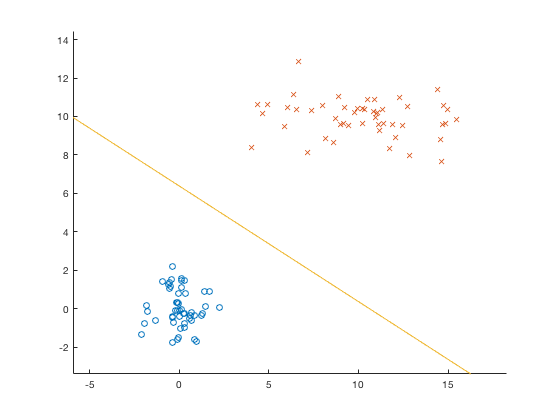
\includegraphics[scale=0.5]{graphintro.png}
\end{frame}


\begin{frame}
\begin{itemize}
\item entr�e: n points $x_i\in \R^n$, d'�tiquettes $y_i\in \{ -1,1\}$
\item sortie: $w\in \R^n$ tel que le signe de $w^Tx_i$ soit l'�tiquette de $x_i$
\end{itemize}
\end{frame}


\section{Formalisation du probl�me}

\begin{frame}
\frametitle{SVM: cas s�parable}
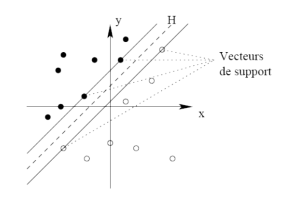
\includegraphics{marge_dure.png}
\end{frame}

\begin{frame}
\frametitle{SVM: cas s�parable}
On maximise l'�cart entre deux hyperplans parall�les qui s'appuient sur des points de chaque cat�gorie.

Ainsi on maximise $\frac{1}{\| w\|_2}$ o� $w\in \R^n$ avec $y_i(w^Tx_i)\ge 1$ pour $1\le i\le n$.

Cela revient � minimiser $\| w\|_2$ ou encore $\frac{1}{2}\| w\|_2^2$ sous les m�mes contraintes.
\end{frame}


\begin{frame}
\frametitle{SVM: cas non s�parable (marge souple)}
minimiser $\frac{1}{2}\| w\|_2^2+C1^Tz$ 

sous les contraintes $y_i(w^Tx_i)\ge 1-z_i$ et $z_i\ge 0$ pour $1\le i\le n$
\end{frame}


\section{R�solution}

\subsection{M�thode barri�re}

\begin{frame}
On minimise $f(w,x)=t(\frac{w^Tw}{2}+C1^Tz)-\sum\limits_{i=1}^m log(z_i)-\sum\limits_{i=1}^m log(y_i(w^Tx_i)-1+z_i)$
\end{frame}

\begin{frame}
\frametitle{M�thode de Newton: $x_{k+1}=x_k-\nabla ^2 f^{-1}\nabla f$}
Pour le gradient $\nabla f$,
\begin{itemize}
\item[$\bullet$] $\frac{\partial f}{\partial w_i}=tw_i-\sum\limits_{k=1}^m \frac{y_kx_k^i}{y_k(w^Tx_k)-1+z_k}$
\item[$\bullet$] $\frac{\partial f}{\partial z_i}=tC-\frac{1}{z_i}-\frac{1}{y_i(w^Tx_i)-1+z_i}$
\end{itemize}

Pour la hessienne $\nabla ^2 f$,
\begin{itemize}
\item[$\bullet$] $\frac{\partial ^2 f}{\partial w_i\partial w_j}=t \delta_{i=j}+\sum\limits_{k=1}^m \frac{x_k^ix_k^j}{(y_i(w^Tx_i)-1+z_i)^2}$
\item[$\bullet$] $\frac{\partial ^2 f}{\partial w_i\partial z_j}=\frac{y_jx_j^i}{(y_j(w^Tx_j)-1+z_j)^2}$
\item[$\bullet$] $\frac{\partial ^2 f}{\partial z_i\partial z_j}=\delta_{i=j}(\frac{t}{z_i^2}+\frac{1}{(y_i(w^Tx_i)-1+z_i)^2})$
\end{itemize}
\end{frame}


\subsection{CVX}

\begin{frame}
CVX est nettement plus rapide quand on augmente la dimension ou le nombre de points.

En effet $\nabla ^2 f$ est de taille $(m+n)\times (m+n)$.
\end{frame}


\subsection{Coordinate Descent Method}

\begin{frame}
\frametitle{Coordinate Descent Method}
\begin{itemize}
\item Descente de Gradient Stochastique: on minimise selon une donn�e � chaque �tape.
\item Coordinate Descent Method: on minimise selon une direction � chaque �tape
\end{itemize}
\end{frame}


\section{Tests}

\begin{frame}
On a test� sur diff�rents exemples en 2D.

Ici: deux gaussiennes d'esp�rances $\begin{pmatrix} 0 \\ 0 \end{pmatrix}$ et $\begin{pmatrix} 7 \\ 0 \end{pmatrix}$ et de covariances $\Sigma_1=I_2$ et $\Sigma_2=\begin{pmatrix} 8 & 0 \\ 0 & 1 \end{pmatrix}$.
\end{frame}

\begin{frame}
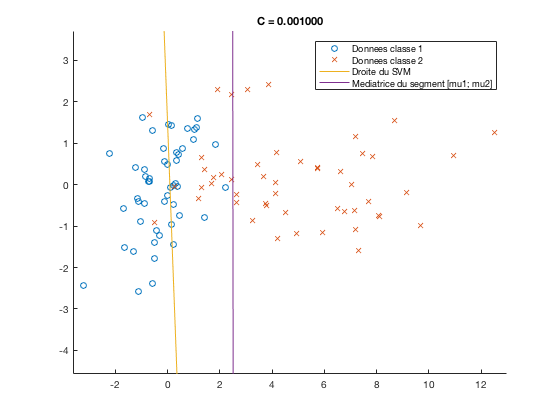
\includegraphics[scale=0.5]{points0dot001.png}
\end{frame}

\begin{frame}
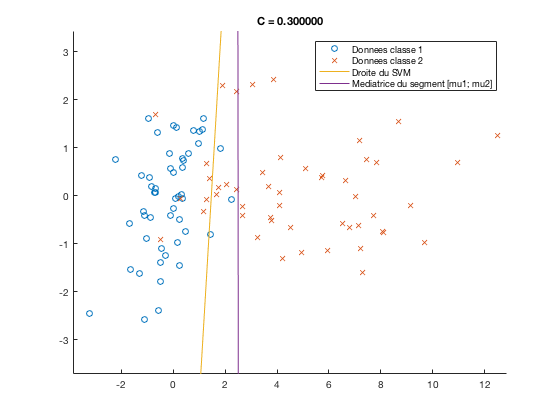
\includegraphics[scale=0.5]{points0dot3.png}
\end{frame}

\begin{frame}
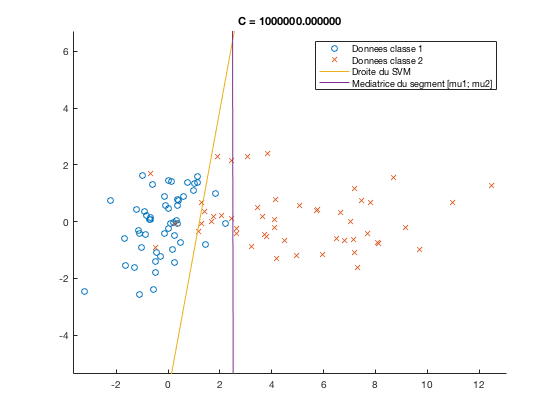
\includegraphics[scale=0.5]{points1000000.png}
\end{frame}

\begin{frame}
\frametitle{Analyse selon C}
\begin{center}
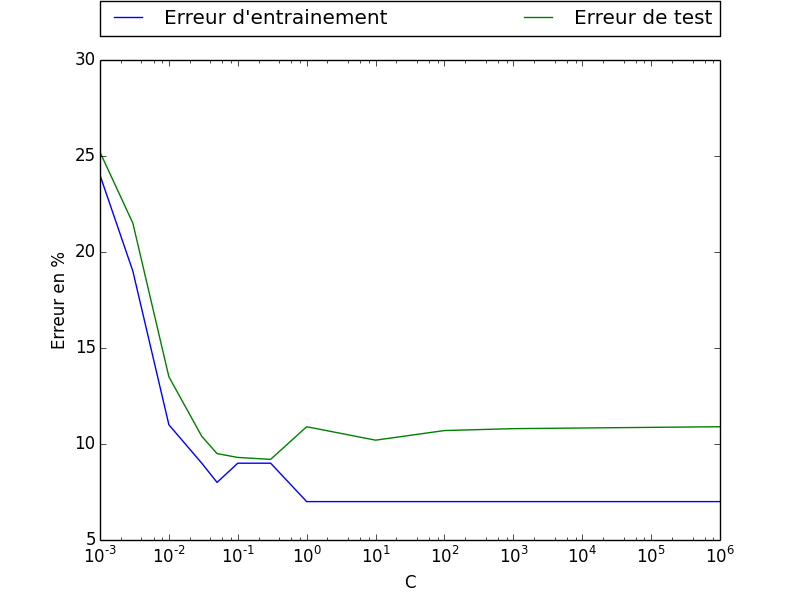
\includegraphics[scale=0.45]{variation_C.png}
\end{center}
\end{frame}

\begin{frame}
\frametitle{Duality gap}
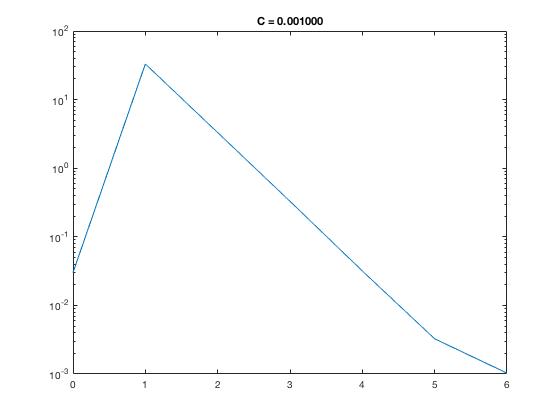
\includegraphics[scale=0.5]{gap0dot001.png}
\end{frame}

\section{Conclusion}

\begin{frame}
\frametitle{Conclusion}

\end{frame}

\end{document}